\usetikzlibrary{arrows.meta}
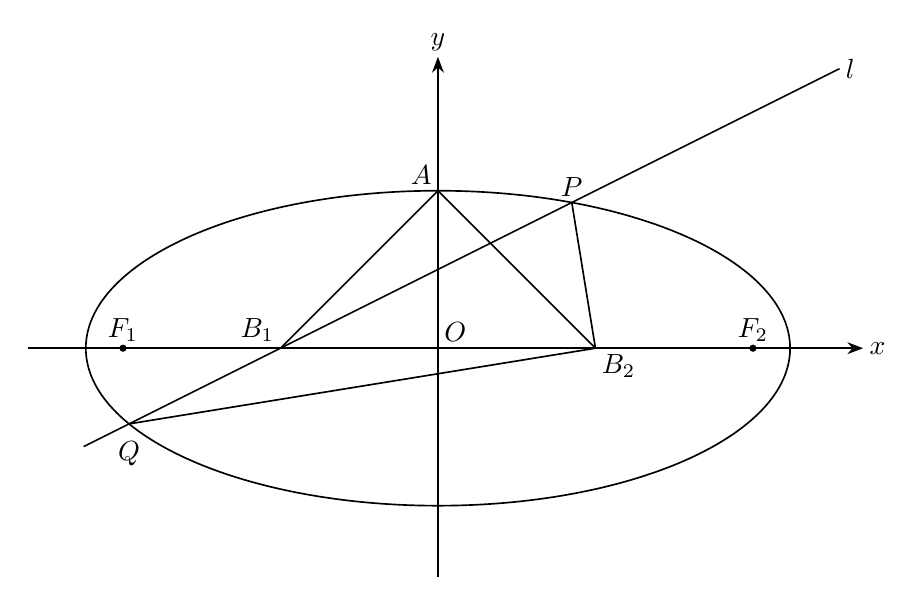
\begin{tikzpicture}[x=1cm,y=1cm,line width=.6pt,>=Stealth,font=\normalsize]
\coordinate (O)  at (0,0);
\coordinate (A)  at (0,2);
\coordinate (F1) at (-4,0);
\coordinate (F2) at (4,0);
\coordinate (B1) at (-2,0);
\coordinate (B2) at (2,0);
\coordinate (P)  at (1.6998023646,1.8499011823);
\coordinate (Q)  at (-3.9220245868,-0.9610122934);
\draw[->] (-5.2,0)--(5.4,0) node[right,inner sep=2pt] {$x$};
\draw[->] (0,-2.9)--(0,3.7) node[above,inner sep=2pt] {$y$};
\draw (O) ellipse [x radius=4.472135955, y radius=2];
\draw (-4.5,-1.25)--(5.1,3.55);
\draw (A)--(B1) (A)--(B2) (B2)--(P) (B2)--(Q);
\fill (F1) circle (1.3pt) (F2) circle (1.3pt);
\node[above left,inner sep=2pt] at (A)  {$A$};
\node[above,inner sep=2pt] at (F1) {$F_1$};
\node[above,inner sep=2pt] at (F2) {$F_2$};
\node[above left,inner sep=2pt] at (B1) {$B_1$};
\node[below right,inner sep=2pt] at (B2) {$B_2$};
\node[above,inner sep=2pt] at (P)  {$P$};
\node[below=5pt,inner sep=1pt] at (Q) {$Q$};
\node[anchor=south west,inner sep=0pt,xshift=2pt,yshift=2pt] at (0,0) {$O$};
\node[right,inner sep=2pt] at (5.1,3.55) {$l$};
\end{tikzpicture}
